% exercise sheet with header on every page for math or close subjects
\documentclass[12pt]{article}
\usepackage[utf8]{inputenc}
\usepackage{latexsym}
\usepackage{multicol}
\usepackage{fancyhdr}
\usepackage{amsfonts}
\usepackage{amsmath}
\usepackage{amssymb}
\usepackage{enumerate}
\usepackage{listings}
\usepackage{graphicx}
\usepackage[parfill]{parskip}

% Shortcuts for bb, frak and cal letters
\newcommand{\E}{\mathbb{E}}
\newcommand{\V}{\mathbb{V}}
\renewcommand{\P}{\mathbb{P}}
\newcommand{\N}{\mathbb{N}}
\newcommand{\R}{\mathbb{R}}
\newcommand{\C}{\mathbb{C}}
\newcommand{\Z}{\mathbb{Z}}
\newcommand{\Pfrak}{\mathfrak{P}}
\newcommand{\Pfrac}{\mathfrak{P}}
\newcommand{\Bfrac}{\mathfrak{P}}
\newcommand{\Bfrak}{\mathfrak{B}}
\newcommand{\Fcal}{\mathcal{F}}
\newcommand{\Ycal}{\mathcal{Y}}
\newcommand{\Bcal}{\mathcal{B}}
\newcommand{\Acal}{\mathcal{A}}

% formating
\topmargin -3.5cm
\textheight 22cm
\textwidth 16.0 cm
\oddsidemargin -0.1cm

% Fancy Header on every Page
\pagestyle{fancy}
\lhead{\textbf{Embedded Systems Problem Set D}}
\rhead{Daniel Schäfer (2549458)\\ Rafael Dewes (2548365)\\ Kevin M\"uller (2550062)}
\renewcommand{\headrulewidth}{1.2pt}
\setlength{\headheight}{110pt}

\begin{document}
\pagenumbering{gobble}
\lstset{language=C++}

\section*{Problem D1}
\subsection*{a)}
\begin{itemize}
\item \textbf{Static hardware redundancy:} Multiple identical modules run in parallel and produce outputs. A voter takes the outputs from the modules and produces a majority value which is good for fault masking. The key difference to dynamic hardware redundancy is that all modules constantly run and produce an output (hot standby) and the fault is not detected but only masked. 

\item \textbf{Dynamic hardware redundancy:} There is one default module that produces an output and several identical ''backup'' modules. A fault detector monitors the output of the currently active module. Upon detecting a fault, a switch is activated and the signal of one of the other modules is used providing a recovery from the error. This allows a detection and localisation of the fault. The main difference to static hardware redundancy is that only the output of one module is used. Therefore, it is possible that all the redundant modules are inactive as long as they are not needed (cold standby).
\end{itemize}
\subsection*{b)}
\begin{itemize}
\item \textbf{Reconnaissance Drone:} The module fails with a chance of $2\%$ which in one year is equivalent to failing $\frac{2}{17520} = 0.00005\%$ in 30 minutes if the module was used for a whole year. However, it is replaced after each flight so the chance of failing is even lower. Since the module is very expensive (and military spending is high enough already) we do not need hardware redundancy in this case.\\
Another reason against redundancy here is that drones have to be very light and oftentimes run on limited energy (batery or solar) which means we have to keep weight and energy consumption of our hardware to a minimum.
\item \textbf{Satellite:} In this case, the probablitity of a single module failing during the mission is quite high (about 22\%). Although the module is expensive it might make sense to order three of them because the cost when the mission fails due to a fault might be a lot higher. A hybrid redundancy approach would be most reliable but we don't have enough modules and spares for that.\\
Whether we choose a dynamic or static approach really depends on the system and the module. If the module is very time critical, a fault detector might be too slow. \\
On the other hand, a TMR has higher energy consumption which might also be problematic for a satelite. Still, the biggest advantage which is why I would choose a dynamic approach with a fault detector with 1 or 2 spares is that we will actually detect the fault and not only mask it. This way, we can report the fault and take actions to fix it. This would not be possible with a TMR.
\item \textbf{Reading-Light:} Since the module is checked daily it is not necessary to use a fault detector. Of course it depends on the budget of the airline but considering the high reliability, probably low weight and the fact that it is not immediately replaced we should buy three units. Using them in a TMR circuit it does not matter if one module fails because the voter will output the value of the two working modules.
\end{itemize}
\section*{Problem D2}
\subsection*{a)}
Ideas for this exercise come from The Byzantine Generals Problem by Marshall Pease and Robert Shostak.
We can generalize the A(1) algorithm to A(m) by keeping the behaviour for A(0) and defining A(m) recursively on a decreasing m. In particular we define:

$A(0)$:
\begin{enumerate}
\item General sends message to all lieutenants.
\item Lieutenant acts according to the generals command.
\end{enumerate}

$A(m)$, for $m>0$:
\begin{enumerate}
\item General sends message to all lieutenants.
\item Each lieutenant acts as general in $A(m-1)$ and distributes the command he received in step 1 to the remaining n-2 lieutenants.
\item Each lieutenant uses the majority of the commands he received from the other lieutenants.
\end{enumerate}
We can think of this propagation of messages as a tree where each rank corresponds to one recursion of the algorithm with the root being the initial general. This general propagates the message to all n-1 lieutenants (step 1.) each represented as a child of the root. Each of them again propagates the message to the remaining $n-2$ lieutenants. This continues recursively until the lieutenants are no longer acting as commander but rather just receive the message and save it. In the last iteration, each commander will receive a message by $n-m$ commanders and decide on the majority of them (step 2). In the second to last recursion, those $n-m+1$ values will be passed on and again evaluated by the majority function. Finally, in the last iteration of this procedure each lieutenant will find the final decision to act on and each of the lieutenants will have the same decision as long as $m < \frac{n}{3}$. See part b) for a correctness argument.

\subsection*{b)}
We want to prove that for $m < \frac{n}{3}$ the above algorithm guarantees that:
\begin{enumerate}
\item If the commander is loyal, the generals should follow the commander's decision.
\item If the commander is a traitor, all loyal generals should decide on the same plan of action, regardless of whether this means attacking or retreating.
\end{enumerate}
Given the recursive definition of the problem/algorithm, it would make sense to do a proof by induction.\\

\textbf{Base case for $m=0$:} 

Algorithm $A(0)$ satisfies the assumption that $0 < \frac{n}{3}$ for all $n>0$ and satisfies both conditions because there is no traitor and each lieutenant will do what the commander says which will be the same for all lieutenants.

\textbf{Inductive step:}

\textit{Condition 1:} We make the inductive step by assuming $A(m-1)$ and showing that $A(m)$ holds. As per definition, assume $A(m-1)$ satisfies condition 1 if $n > 3(m-1)$.\\
A loyal general would run $A(m)$ and send the command to all lieutenants.\\
They would again act as (loyal) general and run $A(m-1)$ and send the command to n-1 lieutenants.\\
$n>3m\\
\implies n-1>3m-1 \\
\implies n-1\geq3m \\
\implies n-1>2m$ for $m\geq1$, thus a majority of the n-1 lieutenants are loyal.

Since each lieutenant uses the majority of the commands he receives from the other lieutenants and n-1 of them are loyal, every lieutenant will use the same command which is the one that the general sent them initially.

\textit{Condition 2:} Condition two follows trivially from condition 1 if the general is loyal. Now, assume that the general is a traitor and $m-1$ lieutenants are traitors. \\
So, the general sends the message to at least $3m-1$ lieutenants which run of which at most $m-1$ are traitors. All of them act as general in $A(m-1)$. However, $3m-1 > 3(m-1)$ which is our initial assumption and thus $A(m)$ also holds and all loyal generals will decide on the same plan of action.

\section*{Problem D3}
\subsection*{a)}
SPI utilizes a synchronized clock signal generated by the master, so all nodes agree on a global timeframe. This would indicate an approach similiar to TDMA. Communication is intiated by the Master node through Slave Select. In the idle state a high voltage level signals the slave node that the line is in a non-transmitting state, which resembles CSMA. Since only one slave select should be driven at a time, SPI avoids collisions from multiple slave nodes, so it would be akin to CSMA/CA. 
Lastly we need to take into account that SPI uses full duplex data transmission. A Slave node must not transmit on its MISO line unless the Master node drives its MOSI line at the same time. This functions as a private time slot for the Slave node.
Therefore the collision treatment in SPI \textbf{uses TDMA}, as collisions can not occur per the specification of SPI.

\subsection*{b)}
The standard SPI protocol does not include a flow control from slave to master, so that we have \textbf{Implicit Flow Control}.

\subsection*{c)}
\begin{figure}[h]
			\centering
			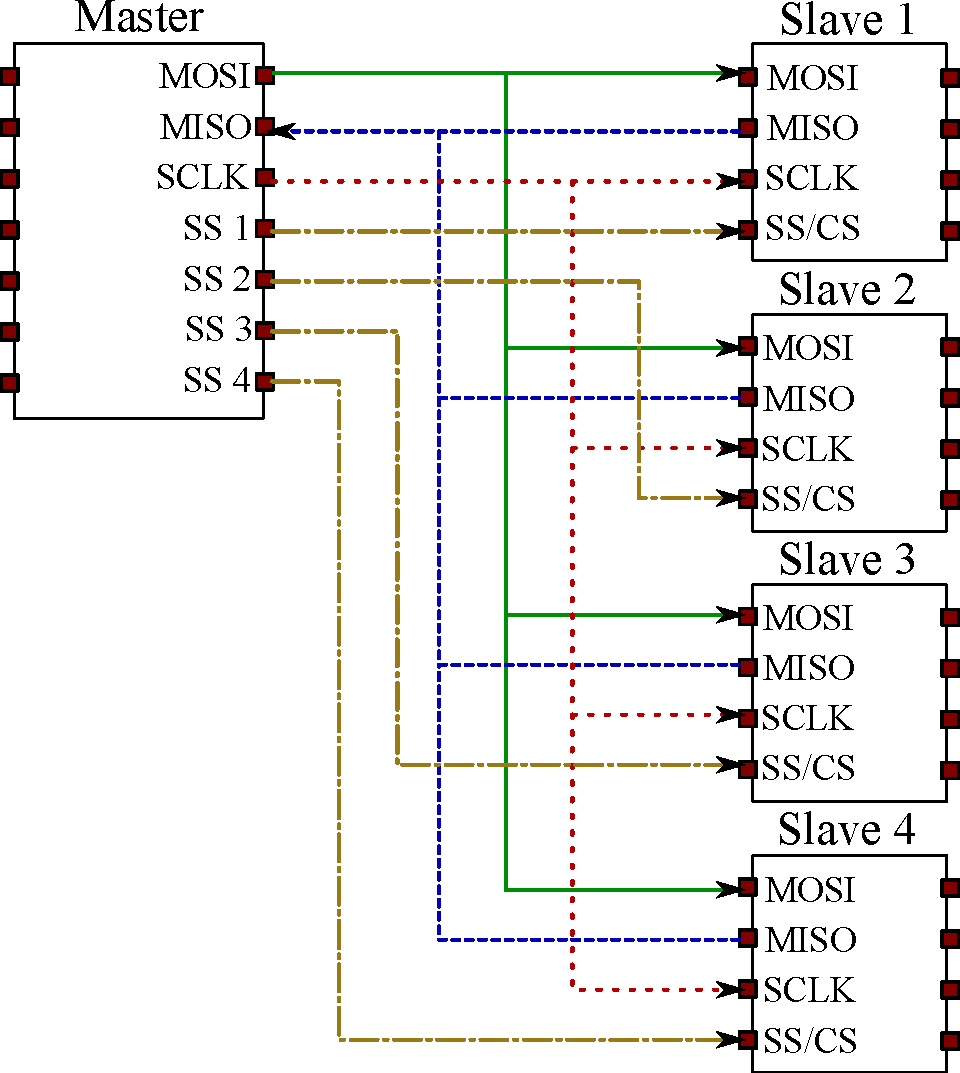
\includegraphics[scale = 0.5]{figures/SPI_drawing}
			\caption{Wiring for one master and four slaves in SPI}
\end{figure}
\begin{figure}[h]
			\centering
			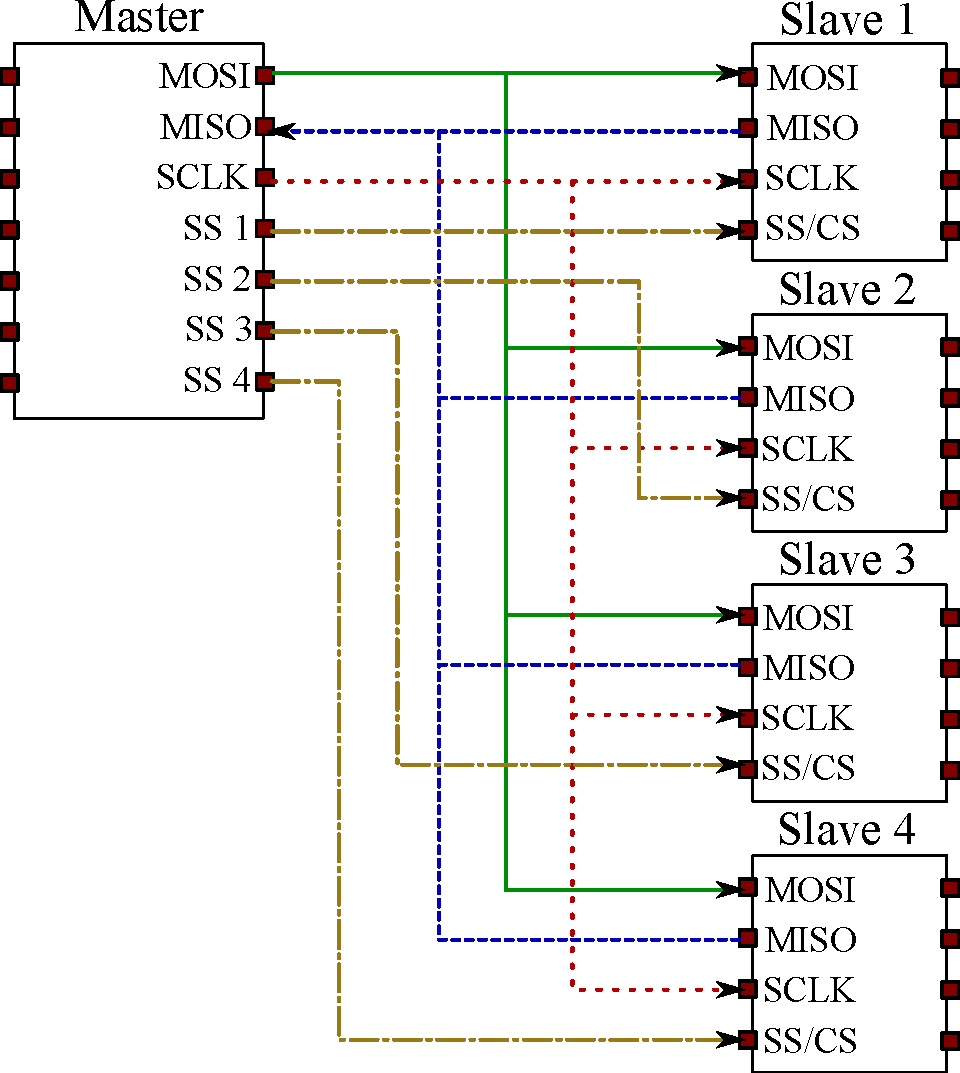
\includegraphics[scale = 0.5]{figures/SPI_drawing}
			\caption{Wiring for one master and four slaves in I$^2$C}
\end{figure}

\end{document}
